\section{Methods}\label{Methods}
In this part we discusse about the methods and the technic of machine learning used in this study
\subsection{Real patient health datasets}\label{datasets}
In order to carry out  our experiments in a real setting we have collected two real world datasets about patients living in Senegal. We describe each of them in the sequel.\\
\textbf{Data collection.} Our first dataset, that we  to refer to it as DT1, contains medical records about patients living in distinct places in Senegal. It has been collected in 2016 during the \textbf{Grand Magal of Touba}  which is one of the most popular religious event in Senegal. Such an event gathers every year several millions of persons that come from various areas around the country \cite{Ch17}.  During the event several fixed and mobile health points are set up to enable the examination and treatment of ill persons. The second dataset, denoted by DT2, has been collected by drawing our attention on medical records about patients living in the same area. We focused on the district of Diourbel,Thies and Fatick \footnote{https://en.wikipedia.org/wiki/Diourbel\_Region} where the prevalence of Malaria is very high and collected patient records from its different health structures. \\
\textbf{Data features. } Table \ref{raw_data} contains the main characteristic of each dataset. Some of these variables (also called features or attributes) include personal data about the patient, but also signs and symptoms of the patient reported by the doctor who treated this later. The other attributes describe clinical data such as information about the doctor's final diagnosis (the patient's disease), the outcome of the Rapid Diagnosis Test and the patient's status (i.e. admission, death or observation). For privacy reasons and certain restrictions in the use of the data, we have ignored patient personal data  during this study.
In addition, we can observe that  both datasets are unbalanced because the proportion of observations per class is largely unequal. As an example for dataset DT1 we have 614 observations in the first class and 5108 observation in the second class. Finally, we remarked that the precision of the Rapid Diagnosis Test is around 90\% for both datasets, meaning that the systematically performed RDT in Senegal is not fully reliable.

%On the other hand,  Figure \ref{missing_values} shows that the raw datasets come %with missing values for  some variables on given observations.
\begin{table*}[!ht]
\centering
  \begin{tabular}{cccccccc}
    \toprule
    \multirow{2}{*}{\textbf{Dataset}} &
      \textbf{Variables}&\textbf{Observations}&
      \multicolumn{2}{c}{\textbf{Variables types}}& \multicolumn{2}{c}{\textbf{Classes}} & \textbf{Precision of RDT}\\
    & & & Numeric & Boolean & Malaria & not Malaria \\
    \midrule
    DT1 &16 & 21083  & 2 &  14& 614&20469 & 90.23\% \\
    DT2 & 16 & 5809 & 2 & 14 & 5108&701 & 90.49\% \\
    \bottomrule
  \end{tabular}
  \caption{Raw Data characteristics}\label{raw_data}
\end{table*}
%\begin{figure*}[!ht]
    %\centering
    %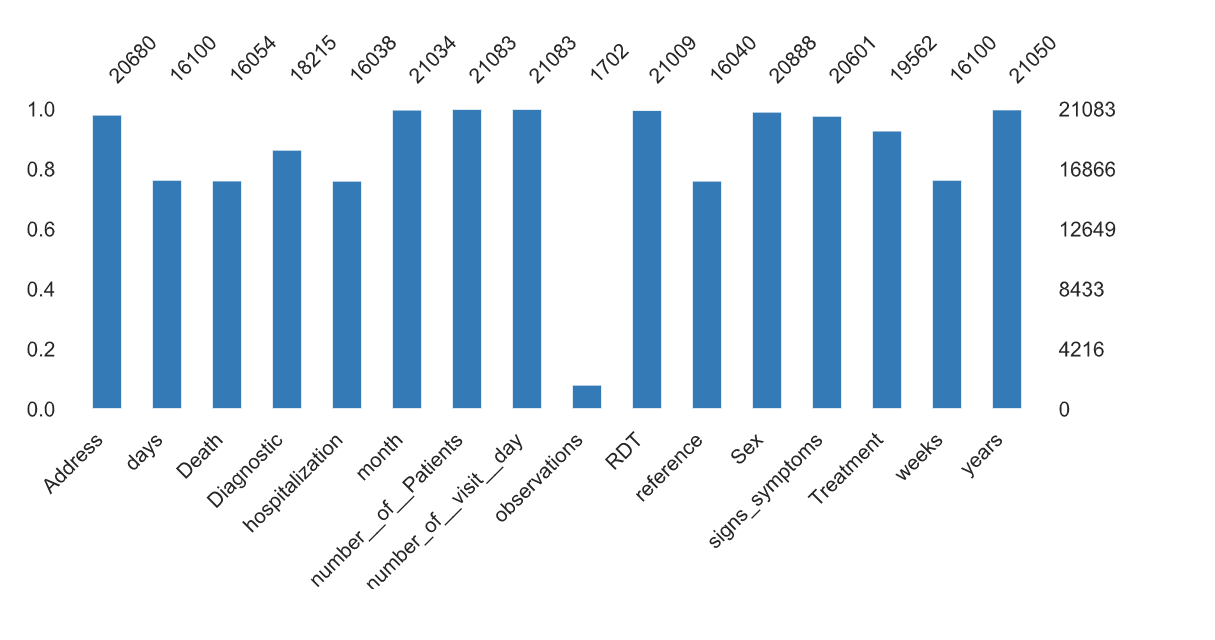
\includegraphics[width=.8\linewidth]{missing_values}
    %\caption{Proportion of missing values per variable}
    %\label{missing_values}
%\end{figure*}
%To resolve the problem of unbalanced datasets and data messness, we followed a data preparation pipeline describe in \cite{mbaye2019towards} in order to fit our datasets into the good format for our experimentation.
%\textbf{Data preparation.}
%\begin{table}[!ht]
%\centering
%\scriptsize
%  \begin{tabular}{ccccccc}
%    \toprule
%    \multirow{2}{*}{\textbf{Dataset}} &
%      \textbf{Variables}&\textbf{Observations}&
%      \multicolumn{2}{c}{\textbf{Variables types}}& \multicolumn{2}{c}{\textbf{Classes}} \\
%    & & & Numeric & Boolean & Malaria & not Malaria \\
%    \midrule
%    DT1 &16 & 61396 & 2 &  14& 30698&30698\\
%    DT2 & 16 & 14336 & 2 & 14 & 7168&7168\\
%    \bottomrule
%  \end{tabular}
%  \caption{Data characteristics after preparation step}\label{synthetic_data}
%\end{table}


From DT1 and DT2 we built three news datasets DT3, DT4 and DT5 data sets as below.\\
\textbf{DT3:}  It is obtained by concatenating the DT1 and DT2 datasets. Thus it concerns 37,175 patients of which 9,837 are diagnosed positive for malaria.\\
\textbf{DT4:} It is obtained by considering the 16,092 patients in the DT2 data set (including 9,223 patients with malaria). Since this DT2 is unbalanced, we randomly selected 2354 patients who tested negative for malaria from the DT1 data set at the end of the rebalance. Thus it concerns 18,446 patients, 9,223 of whom are suffering from malaria.\\
\textbf{DT5:} is obtained by the over sampling of DT1 by the SMOTE method of python. This method consists first of dividing DT1 into two parts, one for training (train set) and the other for testing (test set). The train set being unbalanced, then we apply the SMOTE method to remedy it. Thus we obtain a new train set comprising 30,369 patients, half of whom tested positive for malaria.

\subsection{Experimentation Setting}
In this section data is available for applying classification algorithm. After model creation from training data, classification operation is performed on test data. 
All the performed tests have been done in the same machine and the same operating system. To test the performance of our six chosen ML algorithms, we relied on their Python implementations available through the scikit-learn library. Scikit-learn is an open source simple and efficient tool for predictive data analysis that implements most of the existing ML algorithms

Then some of the most important performance evaluation measures like accuracy, precision, sensitivity, specificity, F-measure and area under ROC curve are evaluated and compared. 
For the details about the description of each parameter of ML we refer to the official documentation of the implementation of these algorithms in scikit-learn7. Concerning the segmentation of both datasets for the training of our ML algorithms and their testing we have considered the stratified-5-fold cross-validation in classification model construction and efficiency evaluation. This method is very useful to handle data with an unbalanced class distribution, increases the validation of classification and prevents from random and invalid results.


